\documentclass[conference]{IEEEtran}
\IEEEoverridecommandlockouts
\usepackage[T1]{fontenc}
\usepackage{mathptmx}
\usepackage{courier}
\usepackage{cite}
\usepackage{amsmath,amssymb}
\usepackage{graphicx}
\usepackage{booktabs}
\usepackage{multirow}
\usepackage{xcolor}
\usepackage{url}
\usepackage[hidelinks]{hyperref}

\newcommand{\sys}[1]{\texttt{#1}}

\begin{document}

\title{DecoyRE: Decoy-Aware Agentic Retrieval\\for Enterprise Knowledge Bases}

\author{\IEEEauthorblockN{Rithika}
\IEEEauthorblockA{\textit{Kantiv}\\
rithika@kantiv.com}}

\maketitle

\begin{abstract}
Enterprise documentation is full of \emph{decoys}: deprecated pages that were never deleted, tables with
near-identical names, wide schemas that chunking splits apart, definitions scattered across several
documents, and questions whose answer does not exist at all. Retrieval-augmented generation (RAG)
returns what is most \emph{similar} to a question, not what is currently \emph{valid}. We present DecoyRE,
a multi-agent pipeline that (i)~automatically curates a raw corpus into a status-aware knowledge bundle,
(ii)~routes each question to a tool plan, (iii)~answers with a tool-using agent over the bundle and a
status-aware hybrid search, and (iv)~verifies the answer with deterministic checks before returning it.
We also release a generated benchmark of 9 corpora (297 documents, 216 questions) covering seven decoy
categories with deterministic, fact-level scoring. With a local 8B model (Qwen3-8B on a laptop CPU),
DecoyRE reaches 77.8\% strict accuracy on 72 questions, statistically on par with dense RAG (75.0\%,
$p=0.82$) while producing no decoy answers, and significantly better than agentic RAG (45.8\%, $p<0.001$)
and a hand-curated knowledge-bundle agent (51.4\%, $p<0.001$). The curator recovers the true status of every
evaluated document (accuracy 1.0 vs.\ 0.50--0.79 for a date-only heuristic). Preliminary ablations show that
the verifier is the most important component, and that the router \emph{hurts}: it mislabels multi-source
definition questions as policy questions and causes most of the system's false abstentions.
\end{abstract}

\begin{IEEEkeywords}
retrieval-augmented generation, enterprise search, LLM agents, knowledge curation, answer verification
\end{IEEEkeywords}

% =====================================================================
\section{Introduction}

Retrieval-augmented generation~\cite{lewis2020rag,gao2023survey} is the default way to connect a
large language model (LLM) to internal company knowledge. Enterprise corpora, however, violate the
assumption that the most similar passage is the right one. A 2023 wiki page titled ``How we calculate
revenue'' is phrased almost exactly like the question ``How do we calculate revenue?'', yet a later decision
record may have replaced it. The table \texttt{orders\_legacy\_pos} may still claim to feed the monthly report.
The column that answers a question may sit 40 lines below the table name, in a different chunk.
We call such documents \emph{decoys}: content that retrieval scores as relevant but that leads to a wrong answer.

LLMs are known to be distracted by irrelevant context~\cite{shi2023distracted}, to under-use information
in the middle of long contexts~\cite{liu2024lost}, and to answer confidently from outdated
knowledge~\cite{kasai2023realtimeqa,vu2024freshllms}. Agentic and self-reflective RAG
variants~\cite{yao2023react,asai2024selfrag,yan2024crag,jeong2024adaptive} add planning or critique, but they
still judge passages by relevance, not by whether a document is currently in force.

Ruiz~\cite{ruiz2026okf} recently argued, with a 7-question demonstration, that an \emph{organizational
knowledge file} (OKF), a hand-written curated bundle of concept pages, beats plain RAG on exactly these
failure modes. That demonstration left two problems open: the bundle had to be written by hand, and the
combined OKF+RAG agent sometimes picked the wrong tool. DecoyRE addresses both.

\noindent Our contributions are:
\begin{itemize}
\item \textbf{A curator agent} that builds the curated bundle automatically from raw documents, combining
rule-based and LLM-based extraction of deprecation evidence, and records each document's status and the
evidence for it.
\item \textbf{A routed, verified answering pipeline} that uses curated concept pages and status-aware search,
followed by deterministic verification (deprecated-citation, grounding, and premature-abstention checks) and one
revision.
\item \textbf{A decoy benchmark} with seven failure categories, three domains, randomized instantiations, and
deterministic fact-level scoring, plus an evaluation of ten systems with bootstrap confidence intervals and
paired exact McNemar tests.
\item \textbf{An honest analysis}, including a negative result: intent routing, a common design choice,
reduced accuracy in our setting.
\end{itemize}

% =====================================================================
\section{Related Work}

\textbf{RAG and hybrid retrieval.} RAG~\cite{lewis2020rag} conditions generation on retrieved passages; surveys
catalogue many variants~\cite{gao2023survey}. Hybrid retrieval combines lexical BM25~\cite{robertson2009bm25}
with dense embeddings~\cite{nussbaum2024nomic}, typically through reciprocal rank fusion~\cite{cormack2009rrf}. All of
these rank by relevance and have no notion of a document being superseded.

\textbf{Agentic and corrective RAG.} ReAct~\cite{yao2023react} interleaves reasoning with tool calls.
Self-RAG~\cite{asai2024selfrag} trains a model to critique its own retrievals, CRAG~\cite{yan2024crag} adds a
retrieval evaluator that triggers corrective actions, and Adaptive-RAG~\cite{jeong2024adaptive} routes queries
by estimated complexity. DecoyRE's verifier is deliberately non-learned: it checks citations against curated
document status and checks that identifiers in the answer appear in retrieved evidence.

\textbf{Structured knowledge for LLMs.} GraphRAG~\cite{edge2024graphrag} builds an entity graph and community
summaries to support global questions. The OKF demonstration~\cite{ruiz2026okf} uses hand-written concept pages.
DecoyRE's bundle sits between the two: unchunked concept pages plus a document-status graph, built automatically.

\textbf{Robustness benchmarks.} RGB~\cite{chen2024rgb} measures noise robustness, negative rejection, and
counterfactual robustness in RAG; SQuAD~2.0~\cite{rajpurkar2018squad2} popularized unanswerable questions;
RealTimeQA~\cite{kasai2023realtimeqa} and FreshQA~\cite{vu2024freshllms} target temporal staleness. Our benchmark
targets staleness and ambiguity \emph{inside} a single organization's corpus, where the corrective evidence
(e.g., a decision record) is itself one of the documents.

% =====================================================================
\section{The DecoyRE Benchmark}

A generator instantiates three fictional companies (retail, SaaS, logistics) with domain specifications
(metrics, business rules, table families, incidents) and writes a raw corpus of wiki pages, schemas,
architecture decision records (ADRs), meeting notes, finance documents, and support tickets. Each domain is
instantiated three times with different random seeds (v1--v3), giving 9 corpora of 33 documents each (297 in
total) and 24 questions per corpus (216 in total). Each corpus has a ground-truth status file
(\emph{current}, \emph{deprecated}, \emph{staging}) used to score curation.

\begin{table}[t]
\caption{Decoy categories (questions per corpus).}
\label{tab:cats}
\centering
\small
\begin{tabular}{@{}p{1.55cm}p{6.1cm}@{}}
\toprule
Category & Planted decoy \\
\midrule
deprecated (3) & Old page phrased like the question; deprecation stated only in a separate ADR; the old page sometimes has a \emph{newer} edit date. \\
validity (3) & Two coexisting definitions; which one is in force. \\
homonym (2) & \texttt{orders}, \texttt{orders\_staging}, \texttt{orders\_v2}, \texttt{orders\_legacy\_pos}; the legacy doc still claims to feed the report. \\
split\_table (4) & Relevant column sits far from the table name in a wide schema. \\
composition (4) & One definition spread over wiki, ADR, meeting note, and finance doc. \\
absence (4) & No answer exists; near-miss documents tempt hallucination. \\
long\_tail (4) & Answer only in a colloquial support ticket. \\
\bottomrule
\end{tabular}
\end{table}

ADR wording comes in three styles: explicit file paths, explicit quoted titles, and implicit references
(``the 2023 analytics write-up''). Rules can parse the first two; the implicit style requires semantic
understanding, which motivates an LLM-assisted curator.

\textbf{Scoring.} Each question lists required facts (identifiers, numbers, ticket IDs, with accepted
alternatives) and decoy facts. An answer is \emph{strictly correct} if all required facts are present, no decoy
fact appears, and the answer is not an abstention. Numbers are matched with digit boundaries (60 does not match
600). For absence questions, an abstention is the only correct answer. We also report \emph{lenient} accuracy
(required facts present), the \emph{decoy rate}, and the \emph{false-abstention rate} on answerable questions.

% =====================================================================
\section{The DecoyRE System}

\subsection{Curator agent}
The curator turns the raw corpus into a bundle in five steps.
(1)~\emph{Self-markers}: documents that declare themselves deprecated.
(2)~\emph{Decision links}: for each ADR and meeting note, a rule extractor resolves sentence-level references
(paths, quoted titles, backticked table names) and classifies them with lexical cues (``supersedes'',
``authoritative'', ``ingestion only''). An LLM extractor receives a catalog of all document paths and titles and
returns JSON lists of deprecated, authoritative, and internal-only documents. The two evidence sets are merged.
(3)~\emph{Resolution}: within each topic, the latest-dated non-deprecated document becomes current and the rest
become stale; in table families, a declared current table makes the other tables stale.
(4)~\emph{Composition}: sentences about the concept found in other non-deprecated documents are attached as
``additional rules''.
(5)~\emph{Emission}: one unchunked concept page per topic and table, an index, and a \texttt{graph.json} recording
each document's status, its successors, and the evidence. Curation runs once per corpus and costs
${\approx}7.3$k LLM tokens.

\subsection{Router, answerer, and verifier}
The \emph{router} classifies the question into one of six intents (definition, table\_choice, schema, incident,
policy, other) with an LLM call in JSON mode, falling back to keyword rules. Each intent maps to a tool plan and
a short hint (e.g., incidents $\rightarrow$ \sys{search\_docs}; definitions $\rightarrow$ \sys{read\_concept}).

The \emph{answerer} is a tool-calling agent (up to six steps) with two tools: \sys{read\_concept}, which returns
a full curated page, and \sys{search\_docs}, a hybrid BM25+dense search with reciprocal rank fusion over
600-character chunks. Search is \emph{status-aware}: deprecated, stale, and internal documents are ranked last
and every hit is labelled with its status and successor.

The \emph{verifier} runs three deterministic checks: (a)~the answer must not cite a document the curator marked
deprecated or stale; (b)~every identifier in the answer (snake\_case names, ticket IDs) must appear in the
retrieved evidence or the question; (c)~an abstention is premature if raw search was never tried. If any check
fails, the answerer reruns once with all tools and the verifier's feedback.

\begin{table*}[t]
\caption{Main results on 72 questions (retail-v1, saas-v1, logistics-v1). Acc: strict accuracy with 95\% bootstrap CI.
Decoy: answers containing a decoy fact. Abst.: correct abstention on absence questions. F-abst.: abstention on answerable
questions. $p$: exact McNemar test vs.\ DecoyRE (wins: questions only DecoyRE / only the baseline gets right).}
\label{tab:main}
\centering
\small
\setlength{\tabcolsep}{3.6pt}
\begin{tabular}{@{}lcccccccccc@{}}
\toprule
System & Acc \% (95\% CI) & Lenient \% & Decoy \% & Abst. \% & F-abst. \% & Prompt tok & LLM calls & Latency (s) & Wins & $p$ \\
\midrule
\sys{rag\_dense}    & 75.0 (63.9--84.7) & 76.4 & 1.7 & 91.7 & 5.0  & 551  & 1.00 & 35.6 & 11 / 9  & 0.82 \\
\sys{rag\_hybrid}   & 70.8 (59.7--80.6) & 72.2 & 3.3 & 75.0 & 5.0  & 576  & 1.00 & 24.7 & 13 / 8  & 0.38 \\
\sys{agent\_search} & 45.8 (34.7--56.9) & 45.8 & 0.0 & 91.7 & 25.0 & 630  & 1.46 & 26.8 & 28 / 5  & $<$0.001 \\
\sys{okf\_rag\_gold}& 51.4 (40.3--62.5) & 51.4 & 0.0 & 100.0& 28.3 & 686  & 1.31 & 17.6 & 25 / 6  & $<$0.001 \\
\textbf{\sys{decoyre}} & \textbf{77.8 (66.7--87.5)} & 77.8 & 0.0 & 91.7 & 13.3 & 1443 & 2.19 & 45.4 & -- & -- \\
\bottomrule
\end{tabular}
\end{table*}

% =====================================================================
\section{Experimental Setup}

\textbf{Systems.} \sys{rag\_dense}: top-5 dense chunks $\rightarrow$ LLM. \sys{rag\_hybrid}: BM25+dense with RRF.
\sys{agent\_search}: ReAct-style agent with search only. \sys{okf\_gold}: agent over the hand-written gold bundle
(upper-bound curation, as in~\cite{ruiz2026okf}). \sys{okf\_rag\_gold}: gold bundle plus search.
\sys{decoyre}: the full system. Ablations remove the verifier, the router, or status-aware ranking, or replace the
curator with a date-only heuristic.

\textbf{Model and hardware.} All systems use Qwen3-8B~\cite{qwen3} (thinking disabled, temperature 0, fixed seed)
and nomic-embed-text~\cite{nussbaum2024nomic} through Ollama, on a laptop CPU (AMD Ryzen~5 5500U, 14\,GB RAM, no
discrete GPU). Everything runs locally, with no data leaving the machine.

\textbf{Statistics.} We report 95\% bootstrap confidence intervals (2{,}000 resamples)~\cite{efron1993bootstrap} and
two-sided exact McNemar tests~\cite{mcnemar1947} on paired per-question correctness. The main comparison uses the
three v1 corpora (72 questions).

% =====================================================================
\section{Results}

\subsection{Main comparison}

Table~\ref{tab:main} and Fig.~\ref{fig:acc} summarize the main comparison. DecoyRE has the highest point
estimate (77.8\%) and is the only system that combines zero decoy answers with accuracy above 70\%. Its advantage
over dense RAG (+2.8 points) is \emph{not} statistically significant ($p=0.82$; 11 vs.\ 9 discordant questions), so
we claim parity with strong RAG baselines, not superiority. DecoyRE is significantly better than agentic RAG
(+32.0 points, $p=0.0001$) and than the agent over the hand-curated gold bundle (+26.4 points, $p=0.0009$).
DecoyRE costs about 2.6$\times$ the prompt tokens of single-shot RAG (1{,}443 vs.\ 551) and 2.2 LLM calls per question.
Per-domain accuracy is 79.2/87.5/66.7\% (retail/SaaS/logistics) for DecoyRE versus 87.5/62.5/75.0\% for dense RAG,
so neither system dominates across domains.

\begin{figure}[t]
\centering
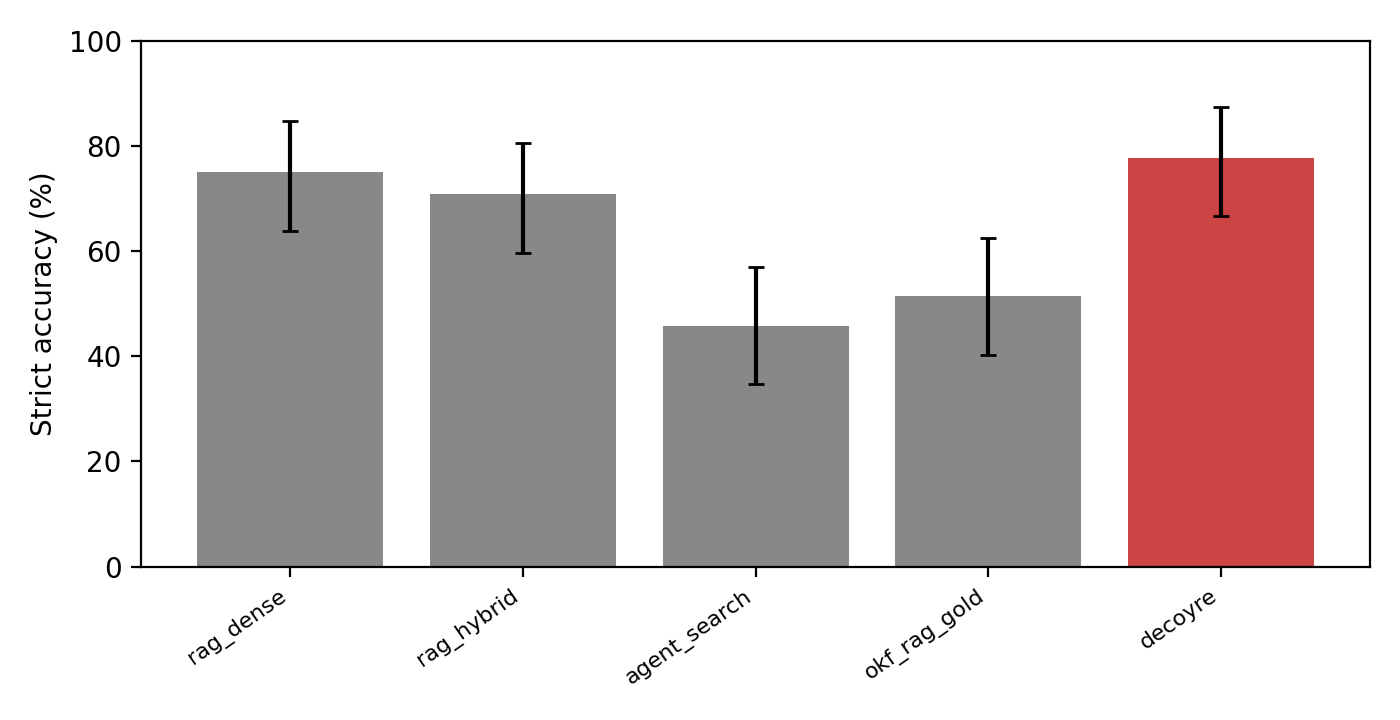
\includegraphics[width=\columnwidth]{figs/fig_accuracy.png}
\caption{Strict accuracy with 95\% bootstrap CIs (72 questions).}
\label{fig:acc}
\end{figure}

\begin{figure}[t]
\centering
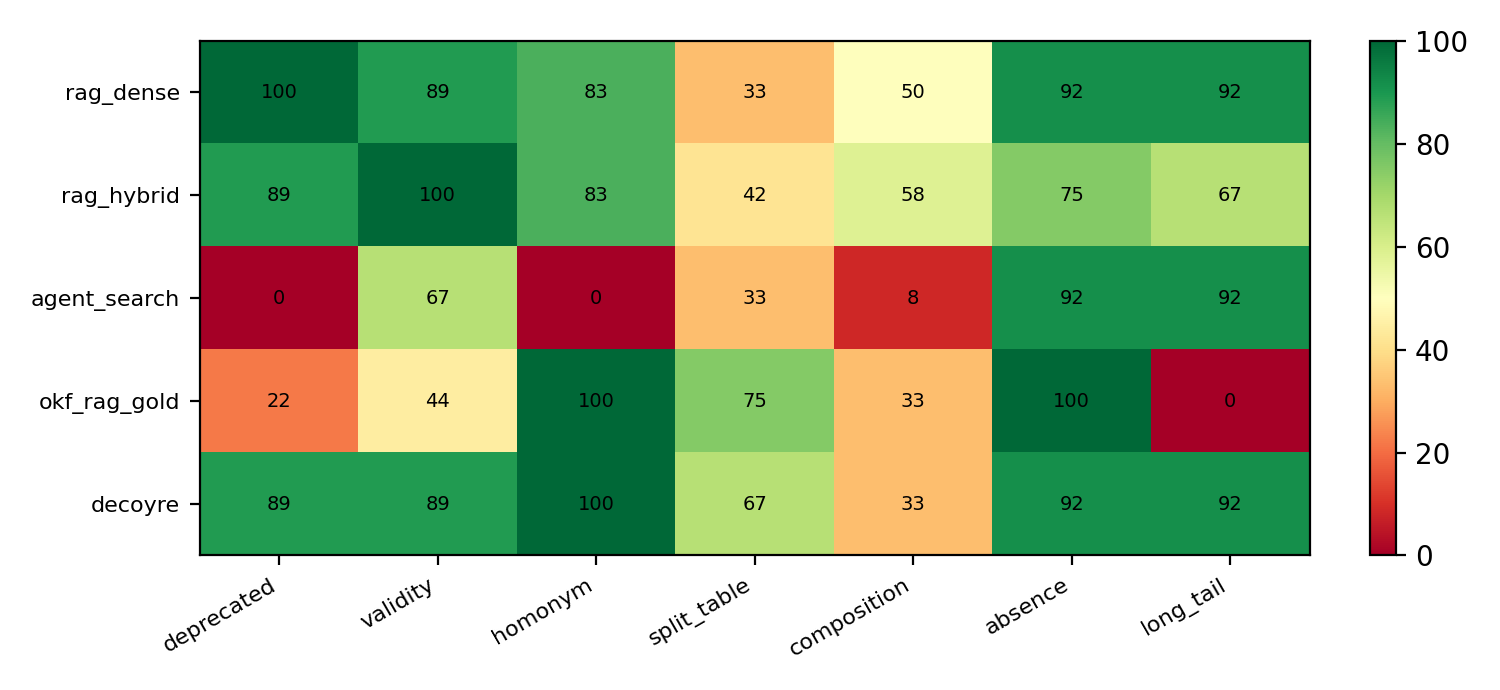
\includegraphics[width=\columnwidth]{figs/fig_categories.png}
\caption{Strict accuracy (\%) by decoy category.}
\label{fig:cats}
\end{figure}

\textbf{Per-category behaviour} (Fig.~\ref{fig:cats}). DecoyRE is the only system at or above 89\% on deprecated,
validity, homonym, absence, and long-tail questions at once. Dense RAG is perfect on deprecated questions, which
indicates that in our generator the deprecation evidence often lands in the same top-5 chunks as the old page;
this makes the benchmark easier for RAG than we intended (Section~\ref{sec:limits}). Every system struggles with
composition (best 58\%, hybrid RAG) and split-table questions (best 75\%, \sys{okf\_rag\_gold}).

\textbf{Why the agent baselines fail.} \sys{agent\_search} answered without calling any tool on 39 of 72
questions (54\%), and \sys{okf\_rag\_gold} on 50 of 72 (69\%), falling back on parametric guesses or citing concept
pages it never opened. This is a tool-use failure of the 8B model rather than a flaw in curated knowledge, and it is
exactly what DecoyRE's verifier catches: it flags answers produced without any tool call and forces a revision. The
verifier fired on 23 of 72 DecoyRE questions.

\textbf{Curation.} The full curator recovers the ground-truth status of every evaluated document in all nine
corpora (accuracy 1.0, 14 documents per corpus). The date-only ablation reaches 0.50--0.93 (0.50/0.64/0.79 on
retail/SaaS/logistics v1), because some deprecated pages carry a newer edit date than their replacement.

\subsection{Preliminary ablations}

\begin{table}[t]
\caption{Preliminary ablations on retail-v1 (24 questions). $p$: exact McNemar vs.\ \sys{decoyre}.}
\label{tab:abl}
\centering
\small
\begin{tabular}{@{}lccc@{}}
\toprule
System & Acc \% & F-abst. \% & $p$ \\
\midrule
\sys{decoyre}               & 79.2 & 15.0 & -- \\
\quad $-$ verifier          & 45.8 & 20.0 & 0.008 \\
\quad $-$ router            & 91.7 & 0.0  & 0.38 \\
\quad $-$ status-aware rank & 79.2 & 15.0 & 1.00 \\
\quad date-only curator     & 62.5 & 10.0 & 0.29 \\
\sys{okf\_gold} (no search) & 37.5 & 35.0 & 0.013 \\
\midrule
\sys{rag\_dense}            & 87.5 & 0.0  & 0.63 \\
\bottomrule
\end{tabular}
\end{table}

The ablation run on all three domains is still in progress; Table~\ref{tab:abl} reports the completed retail-v1 slice
(24 questions), so these numbers are indicative only.
Removing the \emph{verifier} drops accuracy by 33 points ($p=0.008$), making it the most important component.
Replacing the curator with a \emph{date-only} heuristic costs 17 points. \emph{Status-aware ranking} has no measurable
effect, because the agent rarely reaches \sys{search\_docs} on questions where a stale document would win; the curated
pages already carry the status information.

\textbf{The router hurts.} Removing the router \emph{raises} accuracy to 91.7\% and eliminates false abstentions.
The traces show why. On the 72 main questions, the router labelled 18 questions as \emph{policy}: 11 of the 12 absence
questions, but also 7 composition questions. The policy plan exposes only \sys{read\_concept} and
hints ``if no concept covers this policy, say you don't know''. Six of those seven composition questions failed, and
policy routing accounts for 6 of DecoyRE's 8 false abstentions. The router narrows the agent's tool set at exactly the
moment it needs both tools, which is the same wrong-tool problem noted in~\cite{ruiz2026okf}. Exposing all tools and
leaving tool choice to the agent and verifier appears to be the better design.

\subsection{Relation to the OKF demonstration}
Ruiz's 7-question demonstration~\cite{ruiz2026okf} graded RAG, OKF, and OKF+RAG by hand, one question per failure mode.
In the published notes, RAG fails the deprecated and validity questions by quoting the 2023 definition, while OKF fails
the long-tail incident question because it has no search tool, and OKF+RAG wrongly denies that a split-table column exists.
Our larger benchmark reproduces the qualitative pattern: curated knowledge helps on deprecated, validity, and homonym
questions, and a bundle-only agent fails on long-tail questions (\sys{okf\_rag\_gold}: 0\% long-tail). With 72 questions
and paired tests, however, plain RAG turns out much stronger than the 7-question demo suggests, and automatic curation
with verification is what closes the gap.

% =====================================================================
\section{Limitations}
\label{sec:limits}
\textbf{Synthetic, self-authored benchmark.} The same codebase generates the decoys and the curator's lexical rules.
The deprecation wording follows three templates, so the perfect curation accuracy may not transfer to real corpora.
Held-out wording styles and human-written documents are needed.
\textbf{Benchmark difficulty.} Dense RAG is perfect on deprecated questions, so the generator does not yet separate the
systems on the category that motivates the work.
\textbf{Scale.} 72 questions give wide confidence intervals ($\pm$10 points); the v2/v3 corpora (216 questions) and
the full three-domain ablations are running and will tighten them.
\textbf{One model.} All results use Qwen3-8B. The agent baselines' weakness is partly a tool-use weakness of this model;
stronger models may narrow the gap between agentic and pipeline designs.
\textbf{String-match scoring.} Fact matching is deterministic and reproducible but can miss paraphrased correct answers;
lenient and strict accuracy differ by at most 1.4 points here, which suggests this effect is small.

% =====================================================================
\section{Conclusion}
DecoyRE shows that a small, fully local model can answer enterprise documentation questions as accurately as a strong RAG
baseline while never repeating a planted decoy, by curating the corpus automatically and verifying each answer against
document status and retrieved evidence. Automatic curation matched the ground truth on all nine corpora, and the
deterministic verifier was the single most valuable component. Intent routing, by contrast, caused most of the system's
errors. Next steps are to remove the router, evaluate stronger and API-hosted models, and harden the benchmark with
held-out deprecation styles and real enterprise documents.

\section*{Reproducibility}
Code, data generator, curated bundles, per-question answers with tool traces, and scripts for all tables and figures
are included with the project (\texttt{python run.py eval}, \texttt{python run.py report}).

\begin{thebibliography}{99}

\bibitem{lewis2020rag}
P.~Lewis \emph{et al.}, ``Retrieval-augmented generation for knowledge-intensive NLP tasks,'' in \emph{Proc. NeurIPS}, 2020.

\bibitem{gao2023survey}
Y.~Gao \emph{et al.}, ``Retrieval-augmented generation for large language models: A survey,'' arXiv:2312.10997, 2023.

\bibitem{shi2023distracted}
F.~Shi \emph{et al.}, ``Large language models can be easily distracted by irrelevant context,'' in \emph{Proc. ICML}, 2023.

\bibitem{liu2024lost}
N.~F. Liu \emph{et al.}, ``Lost in the middle: How language models use long contexts,'' \emph{Trans. ACL}, vol.~12, 2024.

\bibitem{kasai2023realtimeqa}
J.~Kasai \emph{et al.}, ``RealTime QA: What's the answer right now?'' in \emph{Proc. NeurIPS Datasets and Benchmarks}, 2023.

\bibitem{vu2024freshllms}
T.~Vu \emph{et al.}, ``FreshLLMs: Refreshing large language models with search engine augmentation,'' in \emph{Findings of ACL}, 2024.

\bibitem{yao2023react}
S.~Yao \emph{et al.}, ``ReAct: Synergizing reasoning and acting in language models,'' in \emph{Proc. ICLR}, 2023.

\bibitem{asai2024selfrag}
A.~Asai, Z.~Wu, Y.~Wang, A.~Sil, and H.~Hajishirzi, ``Self-RAG: Learning to retrieve, generate, and critique through self-reflection,'' in \emph{Proc. ICLR}, 2024.

\bibitem{yan2024crag}
S.-Q. Yan, J.-C. Gu, Y.~Zhu, and Z.-H. Ling, ``Corrective retrieval augmented generation,'' arXiv:2401.15884, 2024.

\bibitem{jeong2024adaptive}
S.~Jeong, J.~Baek, S.~Cho, S.~J. Hwang, and J.~C. Park, ``Adaptive-RAG: Learning to adapt retrieval-augmented large language models through question complexity,'' in \emph{Proc. NAACL}, 2024.

\bibitem{ruiz2026okf}
J.~Ruiz, ``rag-vs-okf: Organizational knowledge files versus RAG,'' GitHub repository, 2026. [Online]. Available: \url{https://github.com/JoaquinRuiz/rag-vs-okf}

\bibitem{robertson2009bm25}
S.~Robertson and H.~Zaragoza, ``The probabilistic relevance framework: BM25 and beyond,'' \emph{Found. Trends Inf. Retr.}, vol.~3, no.~4, pp.~333--389, 2009.

\bibitem{nussbaum2024nomic}
Z.~Nussbaum, J.~X. Morris, B.~Duderstadt, and A.~Mulyar, ``Nomic Embed: Training a reproducible long context text embedder,'' arXiv:2402.01613, 2024.

\bibitem{cormack2009rrf}
G.~V. Cormack, C.~L.~A. Clarke, and S.~Buettcher, ``Reciprocal rank fusion outperforms Condorcet and individual rank learning methods,'' in \emph{Proc. SIGIR}, 2009.

\bibitem{edge2024graphrag}
D.~Edge \emph{et al.}, ``From local to global: A graph RAG approach to query-focused summarization,'' arXiv:2404.16130, 2024.

\bibitem{chen2024rgb}
J.~Chen, H.~Lin, X.~Han, and L.~Sun, ``Benchmarking large language models in retrieval-augmented generation,'' in \emph{Proc. AAAI}, 2024.

\bibitem{rajpurkar2018squad2}
P.~Rajpurkar, R.~Jia, and P.~Liang, ``Know what you don't know: Unanswerable questions for SQuAD,'' in \emph{Proc. ACL}, 2018.

\bibitem{qwen3}
Qwen Team, ``Qwen3 technical report,'' arXiv:2505.09388, 2025.

\bibitem{efron1993bootstrap}
B.~Efron and R.~J. Tibshirani, \emph{An Introduction to the Bootstrap}. New York, NY, USA: Chapman \& Hall, 1993.

\bibitem{mcnemar1947}
Q.~McNemar, ``Note on the sampling error of the difference between correlated proportions or percentages,'' \emph{Psychometrika}, vol.~12, no.~2, pp.~153--157, 1947.

\end{thebibliography}

\end{document}
